\documentclass{beamer}
\mode<presentation>
\usepackage{amsmath}
\usepackage{amssymb}
%\usepackage{advdate}
\usepackage{adjustbox}
\usepackage{subcaption}
\usepackage{enumitem}
\usepackage{multicol}
\usepackage{mathtools}
\usepackage{listings}
\usepackage{url}
\usepackage{hyperref}
\def\UrlBreaks{\do\/\do-}
\usetheme{Boadilla}
\usecolortheme{lily}
\setbeamertemplate{footline}
{
  \leavevmode%
  \hbox{%
  \begin{beamercolorbox}[wd=\paperwidth,ht=2.25ex,dp=1ex,right]{author in head/foot}%
    \insertframenumber{} / \inserttotalframenumber\hspace*{2ex} 
  \end{beamercolorbox}}%
  \vskip0pt%
}
\setbeamertemplate{navigation symbols}{}

\providecommand{\nCr}[2]{\,^{#1}C_{#2}} % nCr
\providecommand{\nPr}[2]{\,^{#1}P_{#2}} % nPr
\providecommand{\mbf}{\mathbf}
\providecommand{\pr}[1]{\ensuremath{\Pr\left(#1\right)}}
\providecommand{\qfunc}[1]{\ensuremath{Q\left(#1\right)}}
\providecommand{\sbrak}[1]{\ensuremath{{}\left[#1\right]}}
\providecommand{\lsbrak}[1]{\ensuremath{{}\left[#1\right.}}
\providecommand{\rsbrak}[1]{\ensuremath{{}\left.#1\right]}}
\providecommand{\brak}[1]{\ensuremath{\left(#1\right)}}
\providecommand{\lbrak}[1]{\ensuremath{\left(#1\right.}}
\providecommand{\rbrak}[1]{\ensuremath{\left.#1\right)}}
\providecommand{\cbrak}[1]{\ensuremath{\left\{#1\right\}}}
\providecommand{\lcbrak}[1]{\ensuremath{\left\{#1\right.}}
\providecommand{\rcbrak}[1]{\ensuremath{\left.#1\right\}}}
\theoremstyle{remark}
\newtheorem{rem}{Remark}
\newcommand{\sgn}{\mathop{\mathrm{sgn}}}
\providecommand{\abs}[1]{\left\vert#1\right\vert}
\providecommand{\res}[1]{\Res\displaylimits_{#1}} 
\providecommand{\norm}[1]{\lVert#1\rVert}
\providecommand{\mtx}[1]{\mathbf{#1}}
\providecommand{\mean}[1]{E\left[ #1 \right]}
\providecommand{\fourier}{\overset{\mathcal{F}}{ \rightleftharpoons}}
%\providecommand{\hilbert}{\overset{\mathcal{H}}{ \rightleftharpoons}}
\providecommand{\system}{\overset{\mathcal{H}}{ \longleftrightarrow}}
	%\newcommand{\solution}[2]{\textbf{Solution:}{#1}}
%\newcommand{\solution}{\noindent \textbf{Solution: }}
\providecommand{\dec}[2]{\ensuremath{\overset{#1}{\underset{#2}{\gtrless}}}}
\newcommand{\myvec}[1]{\ensuremath{\begin{pmatrix}#1\end{pmatrix}}}
\let\vec\mathbf

\lstset{
%language=C,
frame=single, 
breaklines=true,
columns=fullflexible
}

\numberwithin{equation}{section}

\title{NCERT-12.9.1.7}
\author{Arnav Mahishi \\ Dept. of Electrical Engg.\\IIT Hyderabad.}

\date{\today} 
\begin{document}

\begin{frame}
\titlepage
\end{frame}
\section*{Outline}
\begin{frame}
\tableofcontents
\end{frame}
\section{Problem}
\begin{frame}
\frametitle{Problem Statement}
Solve the differential equation $y^{\prime\prime\prime}+2y^{\prime\prime}+y^{\prime} = 0$ with initial conditions $y\brak{0} = 1$,$y^{\prime}\brak{0} = -1$ , and $y^{\prime\prime}\brak{0} = 1$
\end{frame}
%\subsection{Literature}
\section{Solution}
\subsection{Input Parameters}
\begin{frame}
\frametitle{Input Parameters}
\begin{table}[]
    \centering
    \begin{tabular}[12pt]{ |c| c|}
    \hline
    \textbf{Variable} & \textbf{Description}\\ 
    \hline
    $n$ & Order of given differential equation\\
    \hline
    $y_i$ & $i$th derivative of the function in the equation\\
    \hline
    $c$ & constant in the equation\\
    \hline
    $a_i$&coefficient of $i$th derivative of the function in the equation\\
    \hline
    $\vec{y}\brak{t}$& Vector containing all 1 and $y_i$ from $i=0$ to $i=n-1$\\
    \hline
    $\vec{y}^{\prime}\brak{t}$ & Vector containing 1 and $y^{\prime}_i$ from $i=0$ to $i=n-1$\\
    \hline
    $A$& the coefficient matrix that transforms each $y_i$ to its derivative\\
    \hline
    $h$&the stepsize between each t we are taking\\
    \hline
    $t_o$& The start time from which we are plotting\\
    \hline
    $t_f$& The end time at which we stop plotting\\
    \hline
    \end{tabular}
    \label{tab:my_label}
\end{table}
\end{frame}
\subsection{Laplace Transforms}
\begin{frame}
\frametitle{Laplace Transforms}
We apply the Laplace transform to each term in the equation. The Laplace transforms for the derivatives of $y\brak{t}$ are:
\begin{align}
\mathcal{L}\fbrak{y^{\prime}\brak{t}} &= sY\brak{s} - y\brak{0} \\
\mathcal{L}\fbrak{y^{\prime\prime}\brak{t}} &= s^2Y\brak{s} - sy\brak{0} - y^{\prime}\brak{0} \\
\mathcal{L}\fbrak{y^{\prime\prime\prime}\brak{t}} &= s^3Y\brak{s} - s^2 y\brak{0} - sy^{\prime}\brak{0} - y^{\prime\prime}\brak{0}
\end{align}
\end{frame}
\subsection{Simplification and Substitiution}
\begin{frame}
\frametitle{Simplification and Substitution}
\begin{align}
\brak{s^3 + 2s^2 + s} Y\brak{s} &= s^2 + s \\
Y\brak{s} &= \frac{s^2 + s}{s(s+1)^2}\\
\implies Y\brak{s} &= \frac{1}{s + 1}
\end{align}
Now, take the inverse Laplace transform:
\begin{align}
\mathcal{L}^{-1}\brak{\frac{1}{s + 1}} = e^{-t}
\end{align}
\end{frame}
\subsection{Radius of Convergence}
\begin{frame}
    \frametitle{Radius of Convergence}
    Radius of Convergence:\\
The denominator indicates a pole at $s=-1$.To ensure convergence of the Laplace transform integral, the real part of $s$ must satsify:
\begin{align}
    Re\brak{s}>-1
\end{align}
Since the ROC extends infinitely to the right in the s-plane, the radius of convergence is:
\begin{align}
    R=\infty
\end{align}
\end{frame}
%\section{Plot}
\subsection{Computational Solution}
\begin{frame}[fragile]
\frametitle{Computational Solution}
$y_{i}$ is the $i$th derivative of the function then
\begin{align}
    \myvec{y_{0}^{\prime}\\y_{1}^{\prime}\\y_{2}^{\prime}\\ \vdots\\y^{\prime}_{n-1}}&=\myvec{y_{1}\\y_{2}\\y_{3}\\ \vdots\\ \frac{-\brak{\sum_{i=0}^{i=n-1}a_iy_i}-c}{a_n}}\\
    \implies  \myvec{1\\y_{0}^{\prime}\\y_{1}^{\prime}\\y_{2}^{\prime}\\ \vdots\\y^{\prime}_{n-1}}&=\myvec{1&0&0&\cdots&\cdots&\cdots&\cdots\\0&0&1&0&\cdots&\cdots&\cdots\\0&0&0&1&0&\cdots&\cdots\\0&0&0&0&1&0&\cdots\\ \vdots&\vdots&\vdots&\vdots&\vdots&\vdots&\ddots\\ \frac{-c}{a_n}&\frac{-a_{0}}{a_n}&\frac{-a_{1}}{a_n}&\frac{-a_{2}}{a_n}&\cdots&\cdots&\frac{-a_{n-1}}{a_n}}\myvec{1\\y_{0}\\y_{1}\\y_{2}\\ \vdots\\y_{n-1}}\\
    \implies \vec{y}_k^{\prime}&=A\vec{y}_k
\end{align}
\end{frame}
%\section{Plot}
\subsection{Trapezoidal Rule}
\begin{frame}[fragile]
\frametitle{Trapezoidal Rule}
Using the trapezoidal rule,
\begin{align}
    J &= \int_a^b f\brak{x}\, dx\\
    &\approx h\brak{\frac{1}{2}f\brak{x} + f\brak{x_1} + f\brak{x_2} \cdots + f\brak{x_{n-1}} + \frac{1}{2}f\brak{b}}\\
   \frac{\vec{y}_{k+1}-\vec{y}_k}{h}&=A\cdot\frac{\vec{y}_{k+1}+\vec{y}_{k}}{2}\\
    \xrightarrow{} \vec{y}_{k+1}&=\brak{I-\frac{h}{2}A}^{-1}\cdot\brak{I+\frac{h}{2}A}\cdot\vec{y}_k
\end{align}
\end{frame}
\subsection{Bilinear Transform}
\begin{frame}
    \frametitle{Bilnear Transform}
    Apply Bilinear Transform with $T=h$ on laplace transform above
\begin{align}
    s&=\frac{2}{T}\frac{1-z^{-1}}{1+z^{-1}}\\
    Y\brak{z}&=\frac{1}{\frac{2}{T}\cdot\frac{1-z^{-1}}{1+z^{-1}}+1}\\
    Y\brak{z}&=\frac{1+z^{-1}}{\frac{2}{h}\brak{1-z^{-1}}+\brak{1+z^{-1}}}\\
    \implies Y\brak{z}&=\frac{1+z^{-1}}{\brak{1+\frac{2}{h}}-\brak{1-\frac{2}{h}}z^{-1}}\\
    \implies \text{Taking }\alpha&=\frac{1-\frac{2}{h}}{1+\frac{2}{h}}\\
    \implies Y\brak{z}&=\frac{\brak{1-\alpha}\brak{1+z^{-1}}}{2\brak{1+\alpha z^{-1}}}\\
    \brak{1+\alpha z^{-1}}Y\brak{z}&=\frac{1-\alpha}{2}\brak{1+z^{-1}}\\
\end{align}
\end{frame}
\begin{frame}
Applying Inverse Z transform, we get the following difference equation
\begin{align}
    y_n&=\frac{1-\alpha}{2}\brak{1+y_{n-1}}\\
    \implies y_n&=\frac{2}{1-\alpha}\delta\brak{n}+\frac{2}{1-3\alpha}y_{n-1},\abs{\alpha}<1
\end{align}
The ROC of the z transform is $1$ as $\abs{\alpha}<1$
\end{frame}
\begin{frame}[fragile]
\frametitle{Plot}
When $k$ ranges from $0$ to $\frac{t_o-t_f}{h}$ in increments of $1$, discretizing the steps gives us all $\vec{y}_k$, Record the $y_{0,k}$ for each $k$ we got and then plot the graph. The result will be as given below.\\
\end{frame}
\begin{frame}
\begin{figure}[H]
   \centering
   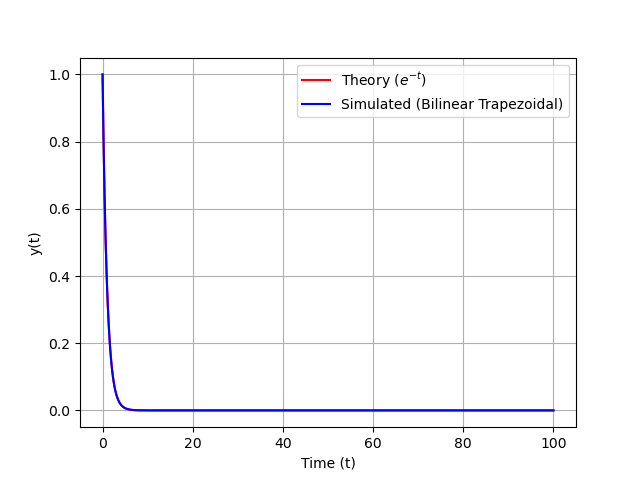
\includegraphics[width=1\linewidth]{../../assignments/Problem 3/figs/fig.png}
   \caption{Comparison between the Theoretical solution and Computational solution}
   \label{stemplot}
\end{figure}
\end{frame}
\begin{frame}
As you can see the graph of bilnear transform is much more accurate compared to the one formed using euler
\begin{figure}[H]
   \centering
   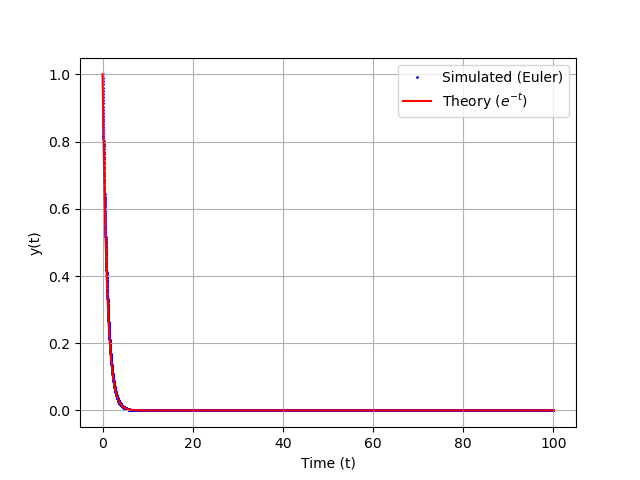
\includegraphics[width=1\linewidth]{../../assignments/Problem 1/figs/fig.png}
   \caption{Eulers Plot}
   \label{stemplot}
\end{figure}
\end{frame}
\end{document}
